\section{Resource allocation for a system following a pipe and filter like architecture}
This section focuses on the main challenges of implementing resource allocation without losing fault tolerance or decoupling between components. Each of the components can be replicated, but replicas of the same component have no means of organizing, they just take the next job that is available in the queue and execute it, no mechanism for distributing the jobs is in place. Replicas of the same component can consume different amounts of system resources, depending on the type of job they are executing, but because they have no possibility to select the jobs they will execute, they just take the next job from the queue, we cannot predict on which of the replicas the job will be executed. Because of this unpredictability, the task of allocating replicas of components to VMs becomes challenging and different methods have been proposed.

Replicas for the "Scanner" component were used as a case study and the following strategies were considered. Jobs present in the queue were marked as H (high), M (medium), L (low) denoting the CPU usage necessary to complete a job. The following methods were proposed in order to extend the system, taking it one step closer to automatic allocation of resources (components).

\subsection{Method 1: Allows the system to balance work in a natural way and not intervene in job allocation}
\label{subsection:method1}
The first strategy was to let the replicas of the "Scanner" component execute whatever job is available in the queue if they are idle. The main advantages of this strategy is that it does not require any changes to the system, so no extra complexity is added. Fig. \ref{fig:randomDistributionsOfTasks} presents the architecture of the first approach. Another advantage is that components are decoupled as envisioned in the initial architecture Fig. \ref{fig:systemArchitecture}.

The main drawback of this approach is that, because balancing is done by chance, in the worst case, the system could be completely unbalanced, some component executing only high intensive CPU jobs while others executing only low CPU intensive jobs. If more than one "Scanner" replicas run on the same VM, than the chances are even lower for this to happen because, even if some component would be "unlucky" enough to only execute CPU intensive jobs, they would be balanced by other components that execute low intensive CPU jobs from the same machine.

\begin{figure}[ht]
\centering
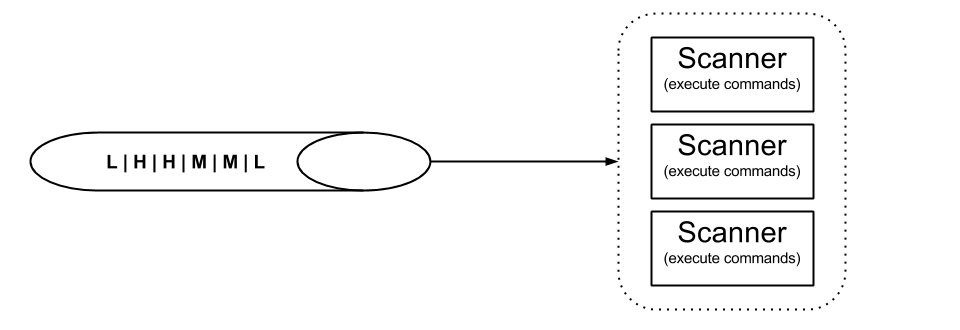
\includegraphics[width=\linewidth]{./img/1_NaturalLoadBalancing.png}
\caption{Random distribution of tasks}
\label{fig:randomDistributionsOfTasks}
\end{figure}

\subsection{Method 2: Assign sizes to jobs and constrain component replicas to execute some type of jobs with a higher priority than others}
\label{subsection:method2}
The second approach Fig. \ref{fig:sizeBaseDistributionOftasks} proposes using some priority scheme inside the "Scanner" component replicas so that we can place "Scanner" replicas on machines that satisfy the required computational needs. For example, if we have a machine with more CPU power, we can allocate "Scanner" replicas that execute CPU intensive jobs. The main advantage of this approach is that we can allocate "Scanner" replicas with different priority schemes to different types of VM's, obtaining a coordinated assignment of component replicas with a knows resource utilization profile. Each replica of the "Scanner" component withdraws messages from the queue, and it makes a decision if it can execute that job or not based on the job type, for example some replicas can only execute CPU intensive jobs (jobs marked with H) while others can execute only low CPU intensive jobs (marked with L). If a replica cannot execute the job, it will just put it back in the front of the queue. Because of this, some messages may spend a very long time in the queue, or even never get executed, if they are always delivered to components that cannot handle them and are put back in front of the queue. Another problem is that the queue is more stressed, because messages are inserted back in the queue if they cannot be executed by a "Scanner" replicas losing the ordering of jobs as well.

\begin{figure}[ht]
\centering
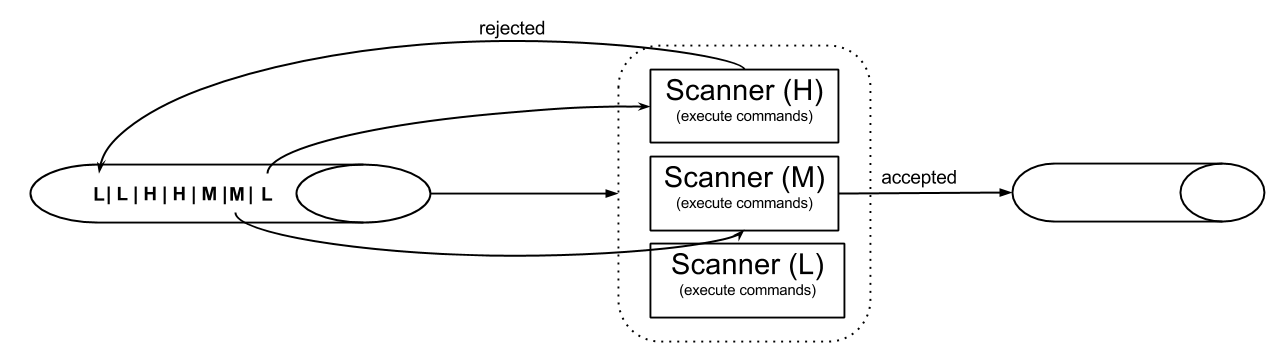
\includegraphics[width=\linewidth]{./img/2_PriorityLoadBalancing.png}
\caption{Size base distribution of tasks}
\label{fig:sizeBaseDistributionOftasks}
\end{figure}


\subsection{Method 3: Create multiple queues deepening on the size of the jobs}

The third method Fig. \ref{fig:multipleQueueDistributionOfTasks} uses a messages queue for every type of job, for out example there are three types of jobs (H, M, L), we need three queues and each "Scanner" replica will have a priority scheme that will dictate the priority it gives to each of the message queues. If the "Scanner" replica does not find messages in the queue with the highest priority, it will take messages from another queue with lower priority. The main advantage of this method, compared with the second method \ref{subsection:method2} is that messages are only withdrawn from one queue reducing the load on the queue, and replicas of components don't have to search for jobs, they can just check if there are jobs available on the queues in the order of their priority scheme. Another advantage is that replicas will not be idle or losing time searching for jobs, they will be executing jobs from queues with low priority if there are no jobs in the high priority queue.

The main drawback is that a new message queue is required if we insert a different type of job, and the "Scanner" replicas will be more complex because they need to keep track of all the queues and the priority schemes.

\begin{figure}[ht]
\centering
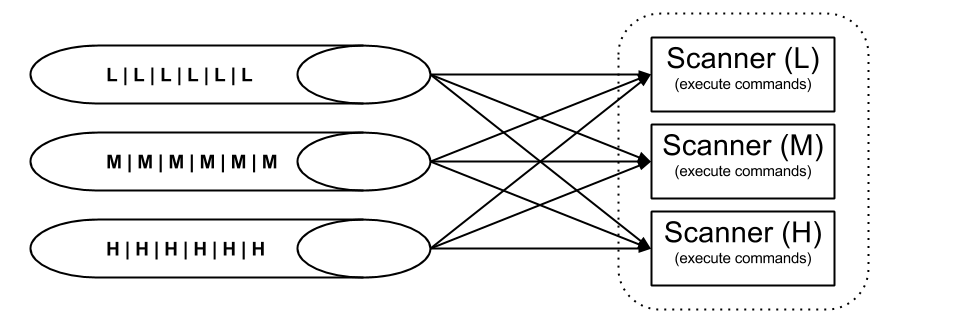
\includegraphics[width=\linewidth]{./img/3_MultipleQueueLoadBalancing.png}
\caption{Multiple queues with multiple size for tasks}
\label{fig:multipleQueueDistributionOfTasks}
\end{figure}

\subsection{Method 4: Use other types of data structure to send the jobs from one component to another}

The forth method Fig. \ref{fig:mapDistributionOfTasks} tries to eliminate all the problems related to job type selection by the "Scanner" replicas by replacing the message queue with a different data structure, in our case a map. In this approach, each "Scanner" replica can inspect all the jobs that can be executed and pick the one best suiting their capabilities.

Although this approach eliminates most of the disadvantages we had when using message queues, it eliminates most of the guarantees that were offered by them as well. Job order is not preserved, the map is a shared by all replicas and operations to it must be serialized to avoid conflicts, or a conflict resolution mechanism should be implemented. Some mechanism for acknowledgment of jobs completion must be implemented in order to avoid losing jobs when components fail.

\begin{figure}[ht]
\centering
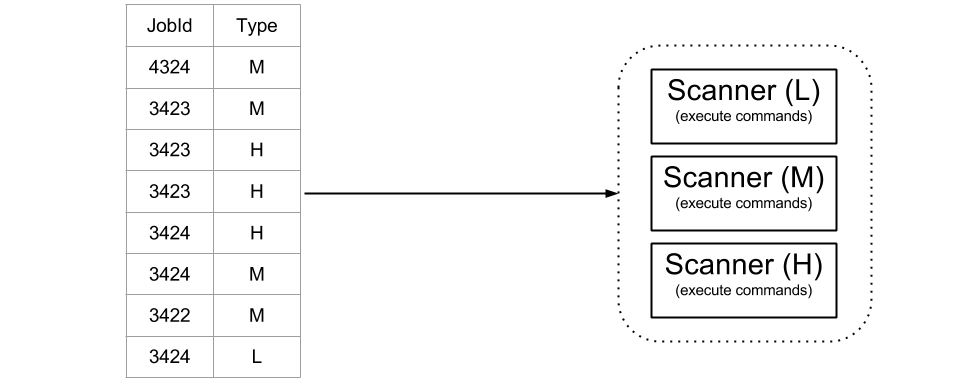
\includegraphics[width=\linewidth]{./img/4_MapOrOtherDataStructureLoadBalancing.png}
\caption{Map with multiple size tasks.}
\label{fig:mapDistributionOfTasks}
\end{figure}

\subsection{Choosing one method}
One of the assumption made at the beginning of this section was that we can determine in advance the CPU usage for jobs, but this can prove to be very difficult in practice because there are more than 3 types of jobs and their CPU usage depends on other factors like network speed and the speed of response for a particular host, network configuration, etc.

As a starting point we chose the method presented in \ref{subsection:method2} because it does not break any of the properties of the system, it can be later extended to any of the more advanced methods and in practice we observed that "Scanner" replicas tend to balanced themselves naturally, without any intervention.